To evaluate the project, I worked with existing REDUCE code for regression testing
but also wrote my own tests in both plain Lisp and RLISP code.
Bracketed Lisp code was useful at the beginning of my project when ParVSL was not
fully functional and I needed unit tests, while RLisp was necessary to write
more complicated code which interfaces with REDUCE.

\section{Single-threaded building of REDUCE}

My project involved modifying a large body of code and it was almost guaranteed
that I would introduce bugs during development. Since the work involves a complex,
multi-paradigm programming language, it is not possible to guarantee to cover all
possible scenarios that might exhibit new bugs. Thankfully, the language and its
direct application are well intertwined, so there is a very large coverage test already
available to demonstrate most functionalities of the language: building REDUCE.

REDUCE consists of around 400 thousand lines of code, and since VSL was built to
run it, all functionality in VSL is being used in REDUCE. In addition to that,
REDUCE comes with a comprehensive suite of regression tests, which were written over the
years to detect bugs in new code. Finally, almost every library in REDUCE contains a
set of tests. These tests involve a large amount of heavy computation, stress testing
many different algorithms, using large amounts of memory and requiring multiple cycles
of garbage collection.

Between building REDUCE and passing its tests, I can detect development bugs and be
confident that ParVSL retains backwards compatibility. Any error while running the code,
or any difference in output between VSL is considered a bug. This approach helped me
find most of the bugs in my code. The disadvantage was that when I had to debug there
was too much code running and it was difficult to pinpoint the source of the problem.

To aid with this, I had multiple stages to build. The first stage was just building
the core, while the second involved building the libraries. If an error showed up while
building a library, most other libraries could be skipped to help pinpoint the problem.
The problem was not completely fixed as just building the core involved running
a very large amount of code, and libraries are also significant in size.

Most of the bugs I could have potentially introduced were data corruption bugs.
I used asserts in various places to try to get the program to crash as soon as possible
and find the issue early. Sometimes I had to introduce a system of binary searching the
problem by trapping the program early and checking for the state of the computation.
I tried to find small tests which would still reproduce the issue, then use the
\texttt{gdb} debugger to step through the code and try to find the errors. I have also used
Valgrind, which offers a large set of tools for detecting undefined behaviour and memory
corruption.

\subsection{Bugs in VSL and REDUCE}

While debugging I discovered some issues in VSL. The language hadn't been tested
extensively until I started working on it. These issues were mostly minor. Some functions
were not present at all and needed to be reintroduced, for example a system function to get
the working directory. There were subtle bugs such as wrong
hard-coded strings and integers. There were multiple issues with floating point manipulation,
again caused by simple human errors (e.g. negated condition being checked). Switching between
output files would lose buffer content. In one place, a value on the heap was not marked
properly, meaning that if a garbage collection was triggered at the right time, it would
be collected prematurely, causing corruption. All these bugs have since been fixed.

REDUCE itself showed multiple cases of sloppy code. Most of the time, the issue was using
a global symbol with a very common name liberally and then behaving weirdly
on clashes. The most striking example was when the RLisp interpreter used the symbol \texttt{x}
during parsing, meaning any tests using the variable \texttt{x} as a free global value
would turn it into a self-reference to code.
Another instance was a name clash in the error handling function, leading to failure
to contain exceptions. While these two cases have been manually fixed, there are many other
such potential problems within the REDUCE packages which will have to be cleaned up.
% Identifying when odd behaviour was down to my code or whether it revealed

\subsection{Benchmarks}

In addition to helping me find issues in ParVSL, building REDUCE also provided a
good performance benchmark. The building process simply runs Lisp and RLisp code so
running it in VSL and ParVSL will showcase the performance difference between the
two in a single-threaded case.

Figure \ref{fig:single-threaded} shows the relative performance of ParVSL compared to VSL.
RCORE is the core of REDUCE, skipping non-essential packages from the build. ALG TEST is
a set of regression tests normally used to check for bugs in the code. INT TEST tests the
symbolic integration package, and provides a good performance benchmark.

\begin{figure}[h]
  \centering
  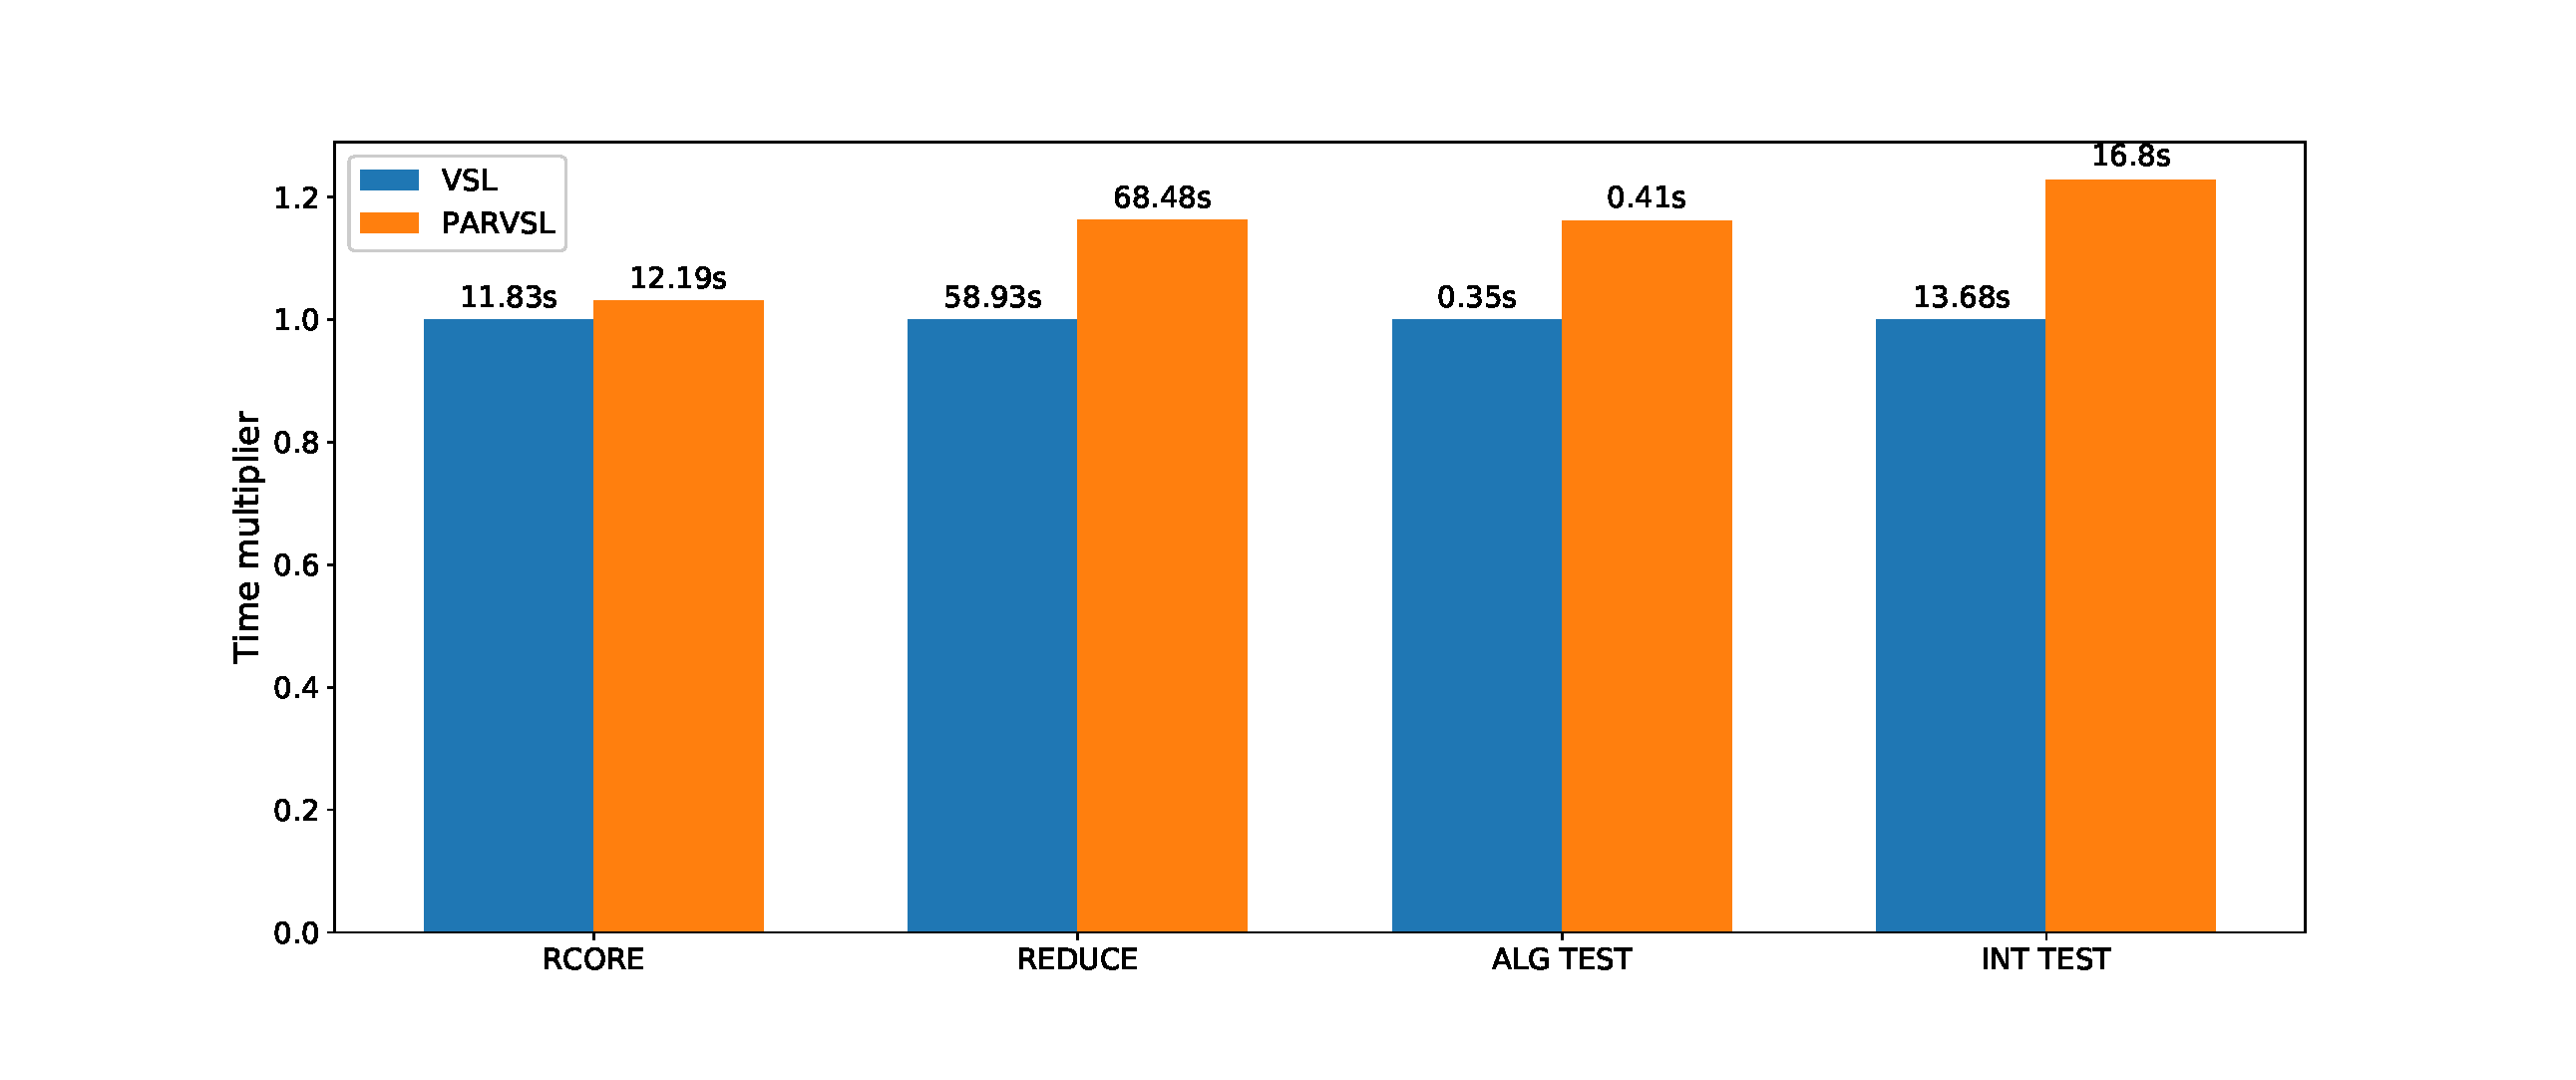
\includegraphics[width=1\linewidth]{single_threaded.eps}
  \caption{Relative performance of ParVSL on single-threaded tests (lower is better).}
  \label{fig:single-threaded}
\end{figure}


A slow-down between 5 and 20 percent can be observed. I have used the GProf \cite{gprof}
tool to profile the code and found the biggest cause of the time difference is the
symbol value extraction mechanism described in \ref{sec:symbols}. In VSL all symbol
values are stored globally with the symbol, whereas ParVSL adds extra book-keeping.
The symbol access function is on the critical path, and slows the code by at least
five percent. This penalty would easily be eliminated in a compiled language, where the
checks for global and fluid variables could be performed statically and optimised away
from the runtime. Other causes of the slowdown are thread-local variables in the interpreter,
which I discuss in section \ref{sec:crossplatform}.

\section{Multi-threading unit tests}

While REDUCE provides a large suite of tests for single-threaded behaviour, I had to come
up with new tests for multi-threading. Before going into larger examples, I started with a small
suite of unit tests in Lisp.

The following test shows multiple threads sharing a variable. They have to acquire
a mutex to prevent a data race. All they do is increment it by one, so the final
value should be equal to the number of calls.

\label{lst:shared-global}
\begin{verbatim}
(global '(x x_mutex))
(setq x 0)
(setq x_mutex (mutex))

(de incr_x ()
  (mutex_lock x_mutex)
  (setq x (add1 x))
  (mutex_unlock x_mutex))

(dotimes (i 10000) (thread '(incr_x)))
(print x)
> 10000
\end{verbatim}

When modifying the garbage collector, I had issues when multiple
threads were initiating it, for example I discovered a deadlock
with my original GC locks (section \ref{sec:gclock}), which I then
quickly fixed. It was easily reproduced with the following test:

\begin{verbatim}
% reclaim forces garbage collection
(dotimes (i 16) (thread '(reclaim)))
\end{verbatim}

Big numbers use continuous areas of memory and can easily
fill in entire segments all at once. The code below simply
raises numbers to a large power in parallel. It helped me discover
that my code was not handling an allocation request being
larger than the segment size.


\begin{verbatim}
% a naive recursive power function
(de pow (a b)
  (cond
    ((zerop b) 1)                  % if b = 0: return 1
    (t (times a (pow a (sub1 b)))) % else: return a * pow(a, b - 1)
  ))

(dotimes (i 1000)
  % raise i^i for really large numbers
  (thread 'pow (list i i)))
\end{verbatim}

These tests, among others, were very helpful in finding bugs
during development. They were added when testing new functionality,
sometimes as a result of finding a bug in a larger example.
They now act as regression tests for ParVSL.

\section{Thread pool}

Once I showed  that ParVSL could run both single-threaded code (i.e. build REDUCE) and pass some
simple tests for multi-threading, I was able to write more complex code using threads.

Spawning hardware threads directly to parallelise each task can be undesirable. The user has
to manage the lifecycle of each thread, making sure to join it and also to manage the number
of available threads on the current hardware directly. Failure to do so will quickly result in
over-subscription of threads. Each thread object comes with its own overhead including a local
stack and operating system handle,

A thread pool is a structure for simplifying parallelism by abstracting away the interaction
with hardware threads. A thread pool consists of a work queue for pending jobs and a number
of worker threads which execute those jobs as they become available. The number of workers
can be kept low so that the program never has to spawn more threads
than the operating system limit, and threads can be reused. Once a thread pool is created,
the user simply needs to submit jobs and they will be automatically parallelised.

\subsection{A thread-safe queue}

The main data structure behind the thread-pool is a thread-safe queue. All threads may push
jobs to this queue and all working threads pop tasks from it to execute. Jobs can be executed
in any order, but I used a FIFO queue so that they would be executed in the order they are submitted,
which seemed the most natural.

We can implement such a queue easily in ParVSL using a mutex and a condition variable.
I wrote the following code in RLisp, since the thread pool will be useful in parallelising
REDUCE code.
We start from a simple queue, with the following functions:

\begin{itemize}
\item \texttt{queue()} creates a new queue
\item \texttt{queue\_push(q, x)} pushes value \texttt{x} to queue \texttt{q}
\item \texttt{queue\_pop(q)} pops and returns the value at the front of the queue
\item \texttt{queue\_empty(q)} checks if the queue is empty
\end{itemize}

A thread-safe queue is simply a wrapper on top of the normal queue:
\begin{verbatim}
procedure safe_queue();
  {queue(), mutex(), condvar()};
\end{verbatim}

We need two procedures: \verb|safe_queue_push(sq, x)| and \verb|safe_queue_pop(sq)|. The latter will
wait if the queue is empty until an element is enqueued. The waiting is done using the condition variable:

\begin{verbatim}
procedure safe_queue_pop(sq{q, m, cv});
begin
  mutex_lock m;

  while queue_empty q do
    % wait for another thread to push an element and notify
    condvar_wait(cv, m);

  res := queue_pop q;
  mutex_unlock m;
  return res;
end;
\end{verbatim}

Now, the push method must notify the condition variable if the queue was empty.
\begin{verbatim}
procedure safe_queue_push(sq{q, m, cv}, x);
begin
  mutex_lock m;
  queue_push(q, x);
  condvar_notify_one cv;
  mutex_unlock m;
end;
\end{verbatim}


\subsection{Managing threads}
\label{ssec:managethreads}

With the queue implemented we can design the worker threads. The starting thread
initialises the queue and starts all the workers as individual threads. It can start
either the maximum number of hardware threads (which can be determined using the
\texttt{hardware\_threads()} function), or a custom count. Each thread is passed a reference to
the thread pool, so it can access the queue. Once the threads are started, they will only
be joined on exit or when the user manually stops the pool.

The mechanism for stopping the queue is a simple atomic flag. Atomics are not offered as
a primitive in ParVSL, but can be easily implemented with a mutex lock. There is no direct
mechanism for interrupting a thread running a task\footnote{C++ does not provide this as a
primitive and indeed if a thread was interrupted in the middle of a system call or while
holding a mutex lock it would cause all sorts of problems.}, but workers can check the flag
every time before taking a new task from the queue.

When the the user tries to stop an empty pool, all
the workers will be in a sleeping state, waiting for the queue condition variable to be
notified and causing a deadlock.

\begin{verbatim}
while atomic_get(run_flag) = 'run do
  // The workers can get stuck here waiting on an empty queue
  job := safe_queue_pop(sq)
  run_job job;
\end{verbatim}

Another idea is to not use a blocking call to pop from the queue, but rather spin:
\begin{verbatim}
while atomic_get(run_flag) = 'run do
  job := safe_queue_try_pop(sq)
  if job then
    // trypop succeeded
    run_job job
  else
    // important to yield here
    thread_yield()
\end{verbatim}

This approach solves the issue, but it is important to note the \verb|thread_yield()| call.
I have implemented \verb|thread_yield()| to directly call the C++ equivalent. This allows the
system to schedule other threads, making sure a waiting worker does not spin the CPU
core to 100\% until forcefully preempted by the OS. It can also cause starvation as it
delays other threads from being scheduled.

\subsection{Waiting for a job's result}
\label{ssec:waitjob}

In ParVSL, the \texttt{thread} function takes another function to execute on the new thread,
along with the arguments for that function. The return value of the function call is
then recovered when joining the thread with \texttt{join\_thread}, enabling thread communication.

When switching from threads to jobs in the thread pool, we want to maintain this functionality,
otherwise the only way to communicate between parallel jobs would be through global state,
which would severely limit its usefulness. Passing arguments for a job is trivial, as they are simply
stored in the safe queue, along with the function to be called. However, returning the result of
a job required extra book-keeping.

Using the primitives in ParVSL, we can implement a \texttt{future} type. A future is a helpful mechanism
that allows us to both wait for a task and obtain its return value. A future starts out as empty.
It can have any number of readers but only one writer. The writer is usually the creator of the future
and will set its value exactly once, at some point after creation. The readers can then try to get the
value inside the future. If the future is fulfilled, the get call returns instantly. Otherwise, it
becomes a blocking call, waiting until the future is set, then returning the respective value.

Implementing a future is similar to the safe queue, using a mutex and a condition variable.
Getting and setting the future requires acquiring the lock. The getter has to wait on the condition
variable if the future is not set. The setter notifies all the getters after setting the value.
The full implementation can be found in Appendix \ref{sec:threadpool-code}.

With the future implemented, we can finish the thread pool, having a mechanism for pushing a job:

\begin{verbatim}
procedure thread_pool_add_job(tp, fn, args):
  fut := future()
  safe_queue_push(tp.safe_queue, {fn, args, fut})
  return fut
\end{verbatim}

The caller can use the future to wait for the result of the job and the workers need to set the future
when finishing a job. Finally, I note that the thread pool must deal with exception handling. The worker threads
need to catch any error while running the job and report it through the future. Initially, I failed to include
it meaning that worker threads unwound unsafely. This lead to the the thread-pool being unable to signal the
thread and fail to terminate. Additionally, threads waiting for the result would also be stuck.

There are many aspects to be considered in the design of a thread pool. I have focused on the main ones, and
this thread pool was sufficient for the rest of evaluation. I have successfully used to to parallelise the
other experiments in this report. However, depending on the task it could be improved upon with more features.
Currently, the number of threads is static, but it could dynamically start and stop threads to accommodate
the workload. An efficient safe queue could be implemented using more granular locking. Furthermore, we could
reduce contention on the queue by having each worker keep its own queue, and the main queue would act as a
dispatcher.

\section{Implementing Parallel Mergesort}

To test the correctness and performance of ParVSL I implemented a few classic algorithms that are relatively
easy to parallelise. Sorting is a particularly good example. Mergesort splits a list in two, sorts each half
recursively, then merges the results to obtain the sorted list. Sorting the individual halves can be done
in parallel.

\begin{verbatim}
tp := thread_pool()

procedure parallel_merge_sort(list):
  if length(list) < 2:
    return list

  xs, ys := split(list)
  sorted_xs_future := thread_pool_add_job(tp, 'parallel_merge_sort, {xs})
  sorted_ys := parallel_merge_sort(ys)
  sorted_xs := future_get(sorted_xs_future)

  return merge(sorted_xs, sorted_ys)
\end{verbatim}

We use the thread pool implemented above to achieve parallelism. Without the thread pool, we would
have to manually manage threads. Using threads here would have resulted in a new thread spawned for
each element in the list. The function would already oversubscribe threads for lists as small as
100 elements. The thread pool only uses a constant number of threads.

\subsection{Dealing with tasks waiting for other tasks}

However, the naive implementation above is incorrect and it will deadlock as soon as the number of
jobs exceeds the number of workers. This highlights a shortcoming of the thread pool. In its current
state is does not handle tasks enqueuing and then waiting for other tasks. In this case, all the workers
will end up waiting for the future (\verb|sorted_xs_future|) without doing any work.

To fix this, I have added extra functionality to the thread pool. An extra procedure \verb|thread_pool_run_job|
can be called by any thread to run one job from the queue. This procedure is implemented similarly
to the worker function, except it only takes at most one job (or none if the queue is empty) from the
queue instead of looping.
This function should be called by any job which is waiting for another job in the thread pool.

I also needed to implement another function for futures \verb|future_try_get|, which only returns the
value in the future if it was fulfilled, without blocking, or indicates failure, without blocking.

Subsequently, I have changed line the \verb|future_get| call above to the following code:
\begin{verbatim}
while null (future_try_get(sorted_xs_future):
  thread_pool_run_job(tp)
\end{verbatim}
Now, workers can start (and finish) other jobs while waiting and will not deadlock.

% \section{{\bfseries\sffamily TODO} Results}
\subsection{Results}

To test the correctness, I simply generate a list of random numbers, then compare the output
to that of the sorting function built in REDUCE. Afterwards, I could test for performance.
I first tuned the parallel version to use the sequential algorithm once if the list is too
small. I found on my machine that around parallelisation became useful once the size of
the list was larger than 1000, and I tuned it to a threshold of 5000. Without this optimisation
the parallel version would spawn too many jobs (as many as \(O(N)\)) and the time book-keeping
would completely eliminate any benefit of multi-threading. Indeed, it runs an order of magnitude
slower on large lists (over 1000 elements). The following table shows the performance improvement
we can gain by increasing the worker count.

\begin{table}[H]
\centering
\begin{tabular}{rrrrr}
& \multicolumn{4}{c}{Number of workers} \\
List size & & & \\
($\times$ 1000) & 1 & 2 & 8 & 16\\
\hline
100  & 2.351 & 1.563 & 1.319 & 1.071 \\
250  & 5.282 & 3.409 & 2.554 & 2.137 \\
500  & 11.152 &  5.850 & 4.906 & 3.995 \\
1000 & 22.840 & 11.706 & 9.054 & 7.514 \\
\end{tabular}
\caption{Parallel merge sort times by number of workers.}
\label{table:parmergesort}
\end{table}

\section{Multiplying polynomials in parallel}

Polynomials are widely used in computer algebra. Being able
to multiply two polynomials is a fundamental problem in computer
algebra with for a plethora of applications ranging from
including symbolic integration and computational geometry,
so speeding it up with multi-threading could prove to be quite valuable.

At the same time, it is relatively easy to split the multiplication
algorithm into multiple independent tasks. All the well-known
multiplication algorithms (i.e. the naive quadratic solution, Karatsuba,
and using the Fast Fourier Transform) have parallel versions \cite[Chapter~30.3]{cormen}.
The latter are mostly used for multiplying numbers, and REDUCE
uses the quadratic algorithm as it is better suited to sparse and
more general multi-variate polynomials.

I wrote a parallel implementation of polynomial multiplication in REDUCE
and ran it in ParVSL. It splits the polynomials into odd and even
terms and thereby splits the problem into four sub-tasks (multiply every combination).
These can be easily computed in separate threads, then joined to obtain the
resulting polynomial. While the small test case only covers uni-variate
polynomials the results I show might reasonably be expected to apply to
more general cases.

% \begin{table}[H]
%   \centering
%   \begin{tabular}{rrrrr}
%   Poly size & VSL & ParVSL \\
%   \hline
%   1000 & 0.660 & 0.480 \\
%   2000 & 1.588 & 0.941 \\
%   3000 & 3.280 & 1.729 \\
%   4000 & 5.486 & 2.834 \\
%   5000 & 8.182 & 4.177 \\
%   \end{tabular}
%   \caption{Parallel multiplication of polynomials vs single-threaded.}
%   \label{tab:parpolymult}
% \end{table}

\begin{figure}[H]
  \centering
  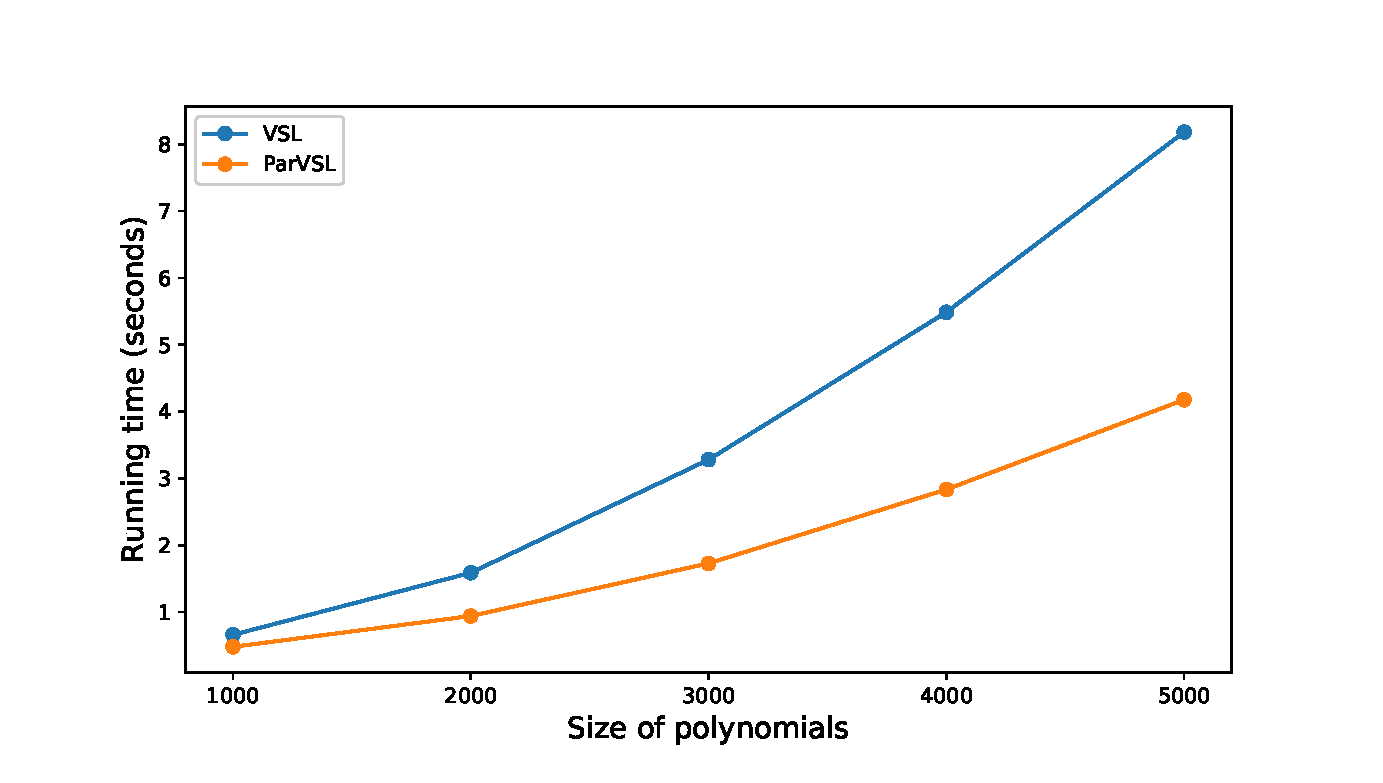
\includegraphics[width=0.8\linewidth]{polymult.eps}
  \caption{Running time of polynomial multiplication in parallel vs single-threaded (lower is better).}
  \label{fig:parpolymult}
\end{figure}

% For small polynomials just gaving the thread infrastructure may
% tend to hurt. After all if you take two quadratics and split them
% into bits to try to multipoly in parallel you are liable to lose!
% For big enough polynomials there can be a saving reasonably consistent
% with the number of threads your CPU can support, and one can then
% suggest that for heavy algebra users that could really help.
% [obviously] if one increases the thread count beyoind the level your
% CPU provides there is no benefit, and possibly ahead of that memory
% bandwidth starts to get saturated, so one does not really expect a
% full factor of 8 on an 8-core machine!
% Your test code does just univariate polys but the results you show
% might reasonably be expected to apply to more general cases, and
% polynomial multiplication is such a fundamental operation in algebra
% that being able to speed it up could really help.

\section{Parallel building of REDUCE}

Most of REDUCE is made up of RLISP code, which can be run in VSL or ParVSL
to generate a build. The process can be separated into two steps:
building the core of REDUCE, and then building all the additional packages.
The core, which I will refer to as RCORE, satisfies most of the dependencies
any of the additional packages need, and only takes a fraction of the time
to build.

\begin{table}[H]
\centering
\begin{tabular}{lr}
 & Time (s)\\
\hline
RCORE & 11.83s\\
REDUCE & 59:93s\\
\end{tabular}
\end{table}

A good use of multi-threading would be to speed up this build time by
arranging to build individual REDUCE packages in parallel. The RCORE base
should still be built sequentially, as it is much more difficult to
separate it into independent tasks. However, the rest of the packages mostly
only have RCORE as a dependency.

I extracted a list of 64 packages to build. The starting point was the
RCORE image. On VSL, I simply ran the building sequentially:

\begin{verbatim}
for package_name in packages do
  build_package package_name;
\end{verbatim}

The total running time was 14.1 seconds. Then, I used the thread pool
to run these builds in parallel:

\begin{verbatim}
tp := thread_pool(hardware_threads());

pack_futures := {};
for package_name in packages do <<
  pack_future := thread_pool_add_job 'build_package {package_name};
  pack_futures := pack_future . pack_futures;
>>;

% We need to ensure all jobs are finished.
for pack_future in pack_futures do
  if (future_get pack_future) != nil do
    print "error building package";
\end{verbatim}

Running this code will initially fail building any package. This is caused
by global side-effects of building the packages. The first issue is that all
packages use global symbols with common names for storage. Any global
symbol used by a package should use a globally unique name, usually by prepending
the package name to the symbol name. Unfortunately, the writers of these packages
didn't always follow good practices. It is outside the scope of this project to
fix all REDUCE packages, however I tried to work my way around that.

I modified the ParVSL code so that when I enable a compilation flag it tracks all
reads and writes to global values of fluid or global symbols. Afterwards, I wrote a Python
script which builds each package individually with the build flag on and saved those
accessed to a file. The script computed all conflicts between packages,
then generated a REDUCE test file which would remove all global access on building the packages:

\begin{verbatim}
% Force conflicting symbols to be fluid.
% Here, global1, global2, etc. are the names of those conflicting symbols
fluid '(global1 global2 ...)
fluid '(store!-global1 store!-global2 ...)

store!-global1 := global1;
store!-global2 := global2;
...

procedure build_package_safe(name);
begin
  % we bind the conflicting variables locally
  scalar global1, global2 ...;

  % restore their original global values inside the local scope
  global1 := store!-global1;
  global2 := store!-global2;
  ...

  build_package(name);
end;
\end{verbatim}

The generated file makes use of the dynamic scoping mechanism in Lisp. When building the package
with \texttt{build\_package\_safe}, all accesses to those global symbols will instead access locally
bound ones. This removes all conflicts between symbol accesses, without needing to modify code in
the REDUCE packages themselves. It also illustrates how in the future REDUCE will need modification
to cope with concurrency.

The second issue I found was that any package can change the access specifier of a global symbol.
One package could make a symbol global, while another tries to bind it locally causing an error.
This issue could not be solved at the Lisp level, so I had to add another temporary flag to the
ParVSL interpreter. Effectively, I disabled globals altogether, and made every global symbol
fluid instead. Fluids allow all the functionality of globals, plus they will allow other threads
to locally bind the name.

Finally, I discovered an inherent design flaw in the Lisp language used by REDUCE which I could not
fix. A feature in REDUCE allows the user to set flags to a symbol. These flags always affect the global
symbol. Many REDUCE packages use this feature, adding, retrieving and removing flags from shared
global symbol names. I could not find a way to around this issue without modifying all of REDUCE.
This meant I was not able to parallelise the building of most REDUCE packages.

Luckily, I did manage to find at least 20 packages which would not conflict in modifying symbol flags.
I parallelised the building of those, the built the other packages sequentially. The resulting
running time was 8.7 seconds (vs 14.1s), a 40\% improvement.
I believe that fixing the issue of shared global names in REDUCE could lead to a significant improvement
of build time when using multi-threading. The speed-up in system rebuild time will be valuable for
developers.

\section{Testing ParVSL on different platforms}
\label{sec:crossplatform}

My benchmarks so far focused on x86 Linux, running
up-to-date compilers. VSL is a cross-platform language which should run on any system as long as the
C++ compiler supports it. ParVSL further requires C++11 support, however at the
time of this writing, the standard is already widely supported on all major platforms.

I tested three major operating systems: Linux, MacOS, and Windows. I also
ran the tests on a Raspberry PI to test it on the ARM platform. Compiling on the Raspberry PI
posed problems even for the single-threaded VSL, as only older compilers are available
there and they exhibiting some bugs in compiling the code and complained about valid code.
The other systems successfully compiled and ran all the code.

The more surprising result is the vast difference in performance between the platforms
when running ParVSL vs VSL. Table \ref{table:cross-platform-reduce} shows the results.

\begin{table}[H]
  \centering
  \begin{tabular}{lrr}
                       & VSL    & ParVSL \\
  \hline
  x86 Linux            &   58s &  1m08s \\
  x86 MacOS            & 1m19s &  3m56s  \\
  x86 Windows (Cygwin) & 1m03s & 10m15s \\
  \end{tabular}
  \caption{Building REDUCE on different platforms in VSL vs ParVSL.}
  \label{table:cross-platform-reduce}
\end{table}

\subsection{Thread-local access performance}

Once observed, this can be verified by trying a trivial test program just referencing a
thread-local variable in a loop. Figure \ref{fig:threadlocal}
shows a huge unexpected extra cost under Cygwin, and noticeable slowdown on the other platforms.

\begin{figure}[H]
\centering
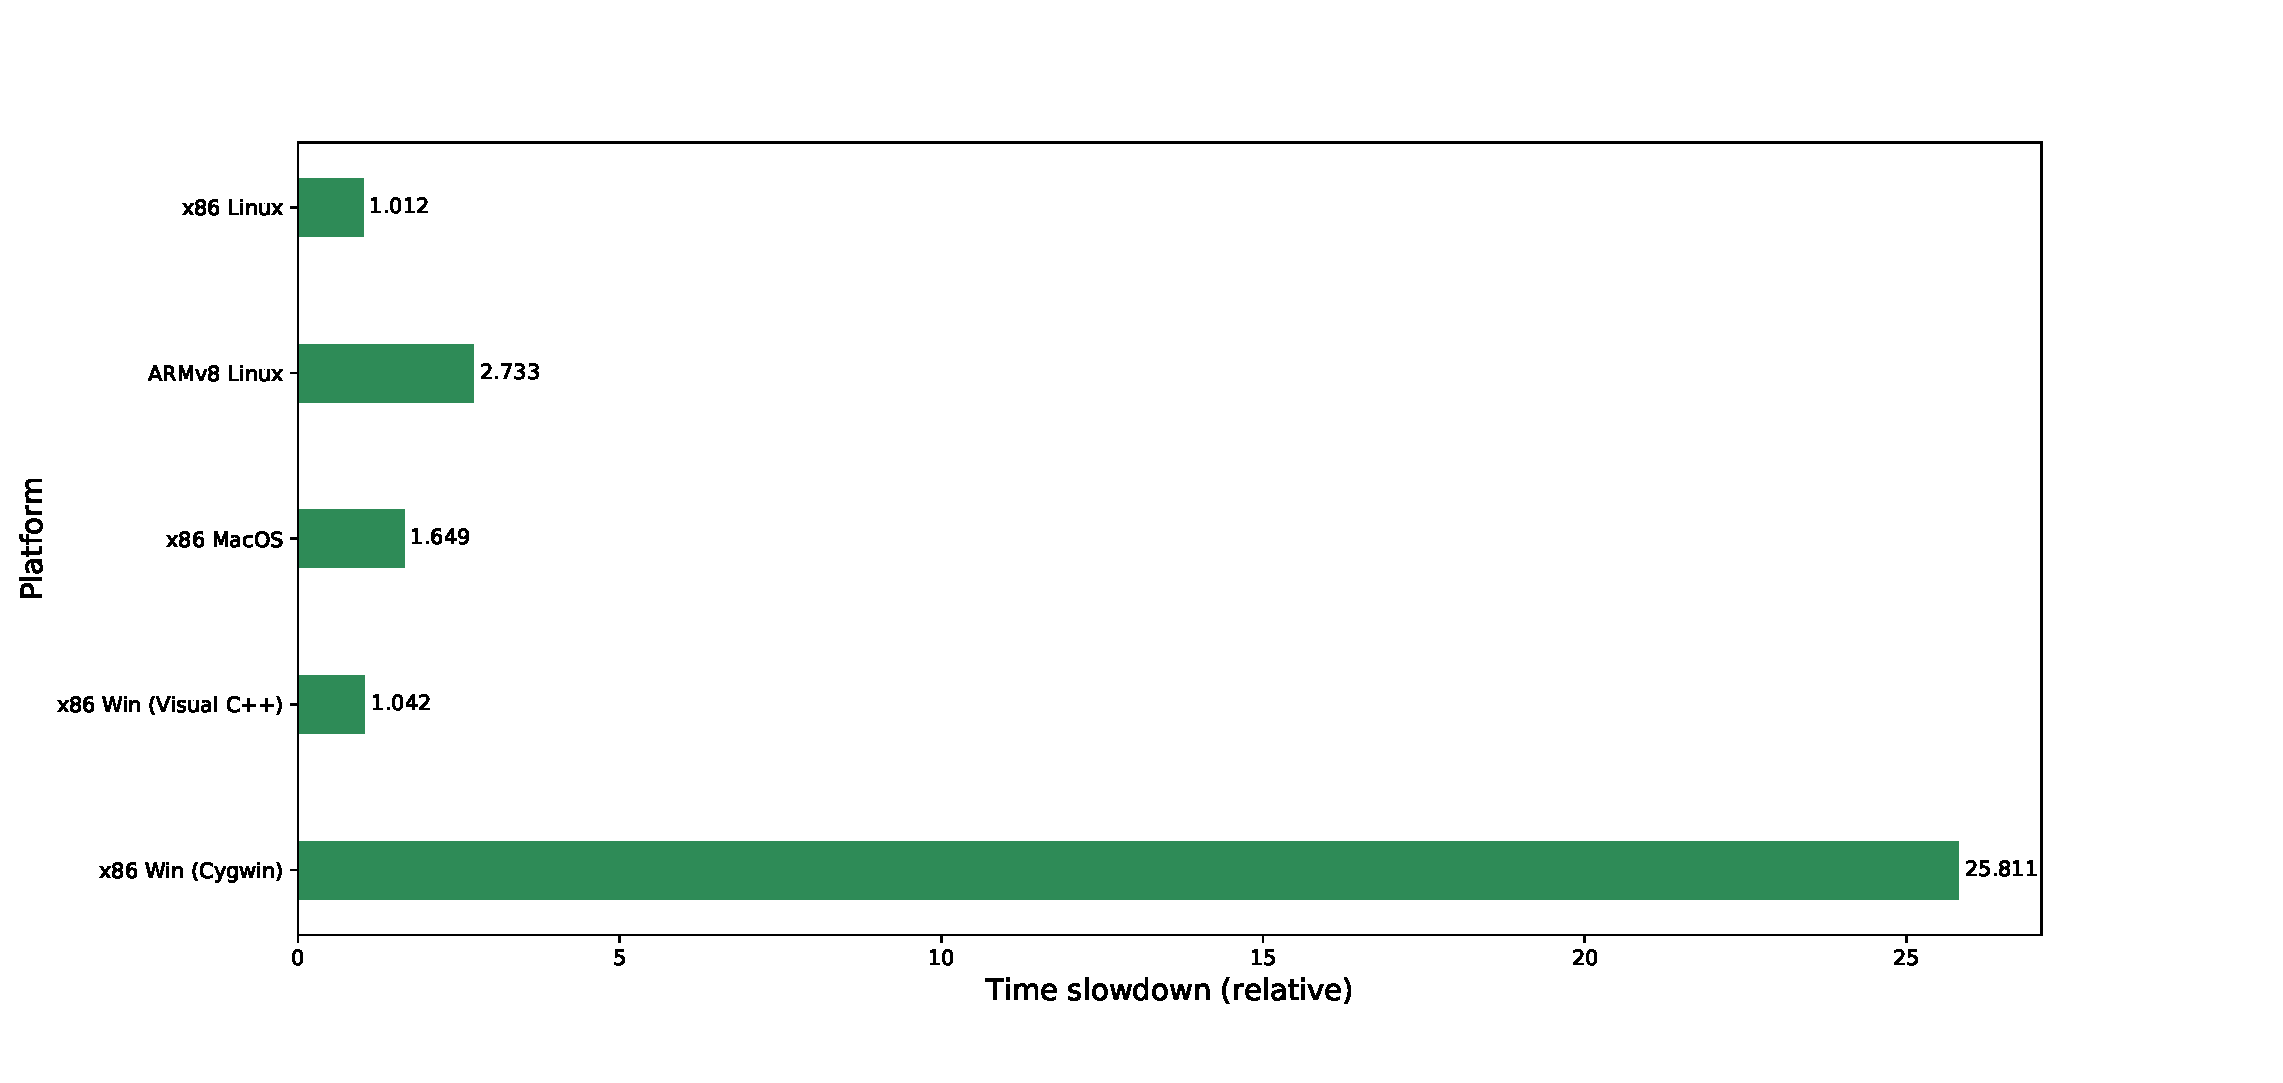
\includegraphics[width=1\linewidth]{thread_local.eps}
\caption{Thread local performance on different platforms (lower is better).}
\label{fig:threadlocal}
\end{figure}

The biggest culprit for the performance impact is the system's thread local storage (TLS)
mechanism. In the best case (i.e. on x86 Linux) a thread-local variable is accessed
similarly to a regular static one. One would hope that Cygwin developers will
implement a more efficient TLS in the future. Currently, the only two platforms
with a negligible TLS slowdown are Linux and (native) Windows.